\documentclass{report}
%
%\IEEEoverridecommandlockouts

\usepackage{ifpdf}
\usepackage{cite}

\usepackage{listings}
\lstset{language=C++}

\ifpdf
  \usepackage[pdftex]{graphicx}
 % \graphicspath{{../pdf/}{../jpeg/}}
  \DeclareGraphicsExtensions{.pdf}
\else
  \usepackage[dvips]{graphicx}
 % \graphicspath{{../eps/}}
  \DeclareGraphicsExtensions{.eps}

\fi
\usepackage{tikz}
\usetikzlibrary{arrows,shapes,backgrounds,matrix,positioning,chains,scopes,patterns}

\usepackage[cmex10]{amsmath}
\usepackage{amssymb}
\interdisplaylinepenalty=2500

%%  header

% \makeatletter
% \def\ps@headings{%
% \def\@oddhead{\mbox{}\scriptsize\rightmark S.~Yang \& R.~W.~Yeung,~Coding for a Network Coded Fountain \hfil \thepage}%
% \def\@evenhead{\scriptsize\thepage \hfil \leftmark\mbox{}}%
% \def\@oddfoot{\scriptsize \@date\hfil DRAFT}%
% \def\@evenfoot{\scriptsize DRAFT\hfil \@date}}
% \makeatother

% \pagestyle{headings}

%\usepackage{algorithmic}

%\usepackage{array}

%\usepackage{mdwmath}
%\usepackage{mdwtab}


\ifpdf
\usepackage[pdftex]{hyperref}
    \hypersetup{
    colorlinks=true,%
    citecolor=black,%
    filecolor=black,%
    linkcolor=blue,%
    urlcolor=blue
  }  
\else

\fi

\setcounter{secnumdepth}{3}


\newtheorem{theorem}{Theorem}
\newtheorem{corollary}[theorem]{Corollary}
\newtheorem{lemma}[theorem]{Lemma}
\newtheorem{proposition}[theorem]{Proposition}

\newtheorem{definition}{Definition}
%\newtheorem{claim}[theorem]{Claim}

%%% Change of equation counter
%\numberwithin{equation}{section}
%\newcommand{\theasection}{\arabic{section}}
%\renewcommand{\theequation}{\theasection.\arabic{equation}}

%%% End of change equation counter
%%% The equation coutner is changes alson in Appendix.


\DeclareMathOperator{\E}{\mathbb{E}}
\DeclareMathOperator{\Gr}{Gr}
%\DeclareMathOperator{\GL}{GL}
\DeclareMathOperator{\Pj}{Pj}
\DeclareMathOperator{\Bi}{I}
\DeclareMathOperator{\rank}{\text{rk}}
%\DeclareMathOperator{\Fr}{Fr}
\DeclareMathOperator{\diff}{d}

%new command

\newcommand{\floor}[1]{\lfloor #1 \rfloor}
\newcommand{\etal}{\textit{et al.}}
\newcommand{\subs}{\text{SS}}
\newcommand{\csub}{\text{C-SS}}

\newcommand{\ffield}{\mathbb{F}}
\newcommand{\ff}{\mathbb{F}}


\newcommand{\lspan}[1]{\langle #1 \rangle}
\newcommand{\tr}{\top}

\newcommand{\gcos}[2]{\begin{pmatrix} #1 \\
#2 \end{pmatrix}_q}
\newcommand{\gco}[2]{\left({}^{#1}_{#2}\right)_q}
\newcommand{\cmat}[2]{\chi^{#1}_{#2}}
%\newcommand{\cmats}[3]{\chi^{#1,#2}_{#3}}
\newcommand{\cmatt}[2]{\zeta^{#1}_{#2}}
\newcommand{\bigO}{\mathcal{O}}

\newcommand{\bG}{\mathbf{G}}
\newcommand{\bB}{\mathbf{B}}
\newcommand{\bX}{\mathbf{X}}
\newcommand{\bY}{\mathbf{Y}}
\newcommand{\bZ}{\mathbf{Z}}
\newcommand{\bH}{\mathbf{H}}
\newcommand{\bR}{\mathbf{R}}
\newcommand{\bzero}{\mathbf{0}}

\newcommand{\uniform}{\text{unif}}
\newcommand{\loc}{\text{LOC}}

\newcommand{\lc}{\mathcal{C}}
\newcommand{\ow}{o.w.}
\newcommand{\bats}{BATS}

\newcommand{\precheck}{\mathbf{P}}
\newcommand{\ldpcnum}{L}
\newcommand{\hdpcnum}{H}
\newcommand{\smnum}{S}
\newcommand{\innum}{I}

%===================
% tikz set
\tikzset{terminal/.style={
% The shape:
rounded rectangle,
minimum size=6mm,
% The rest
very thick,draw=black!50,
top color=white,bottom color=black!20,
font=\ttfamily}}

\tikzset{nonterminal/.style={
% The shape:
rectangle,
% The size:
minimum size=6mm,
% The border:
very thick,
draw=red!50!black!50, % 50% red and 50% black,
% and that mixed with 50% white
% The filling:
top color=white, % a shading that is white at the top...
bottom color=red!50!black!20, % and something else at the bottom
% Font
font=\itshape
}}

\tikzset{endblk/.style={
    rounded rectangle,minimum size=6mm,
    very thick,draw=red!50!black!50,
    top color=white,bottom color=red!50!black!20,
    font=\ttfamily}
    }
\tikzset{process/.style={
    rectangle,minimum size=6mm,
    very thick,draw=black!50,
    top color=white,bottom color=black!20,
    align=center,midway,
    font=\ttfamily}
}
\tikzset{subroutine/.style={
    rectangle,minimum size=6mm,
    very thick,draw=blue!50!black!50,
    top color=white,bottom color=blue!50!black!20,
    font=\ttfamily}
}
\tikzset{conditional/.style={
    shape aspect=3,rounded corners=2mm,
    diamond,minimum size=6mm,
    very thick,draw=green!50!black!50,
    top color=white,bottom color=green!50!black!20,
    align=center,midway,
    font=\ttfamily}
}

\tikzset{skip loop/.style={to path={-- ++(0,#1) |- (\tikztotarget)}}}

\tikzset{point/.style={coordinate},>=stealth',draw=black!70,
  arrow/.style={->},every join/.style={rounded corners},
  hv path/.style={to path={-| (\tikztotarget)}},
  vh path/.style={to path={|- (\tikztotarget)}},
  lyes/.style={label=177:yes},
  lno/.style={label=177:no},
  ryes/.style={label=3:yes},
  rno/.style={label=3:no},
  bno/.style={label=-93:no},
  byes/.style={label=-93:yes},
}

% Draw line annotation
% Input:
%   #1 Line offset (optional)
%   #2 start coordinates
%   #3 Line angle
%   #4 Line length
%   #5 Line label
% Example:
%   \lineann[1]{30}{2}{$L_1$}
\newcommand{\lineann}[5][0.5]{%
    \begin{scope}[rotate=#3, blue,inner sep=2pt]
        \draw[dotted, blue!40] #2 -- +(0,#1)
            node [coordinate, near end] (a) {};
        \draw[dotted, blue!40] #2 ++(#4,0) -- +(0,#1)
            node [coordinate, near end] (b) {};
        \draw[|<->|] (a) -- node[fill=white] {#5} (b);
    \end{scope}
}

%=====================

% correct bad hyphenation here
\hyphenation{op-tical net-works semi-conduc-tor}


\begin{document}
%
\title{Precoded BATS codes}
%

\author{Shenghao Yang\\
  Institute of Network Coding \\The Chinese University of Hong Kong, Hong Kong SAR,
    China \\Email: shyang@inc.cuhk.edu.hk
}

%\author{\IEEEauthorblockN{Shenghao Yang\IEEEauthorrefmark{1}, Jin
%    Meng\IEEEauthorrefmark{2} and En-hui Yang\IEEEauthorrefmark{2}}
%  \IEEEauthorblockA{\IEEEauthorrefmark{1} Department of Information
%    Engineering, The Chinese University of Hong Kong, Hong Kong}
%  \IEEEauthorblockA{\IEEEauthorrefmark{2} Department of Electrical and
%    Computer Engineering, University of Waterloo, ON, Canada} Emails:
%  shenghao.yang@gmail.com, \{j4meng, ehyang\}@uwaterloo.ca }

\maketitle
\tableofcontents

\begin{abstract}
  
\end{abstract}

%\section{Introduction}
%

\chapter{Algorithms}

\section{To Do}

\begin{enumerate}
\item The number of LDPC symbols should be prime.
\item De-randomness of the degree and index generation. Refer to
  \cite[\S 5.3.5]{rfc6330}.
\item De-randomness of the generator matrices. Refer to
  \S\ref{sec:gener-matr-batch}.
\item NC coder starts after receiving enough number of packets of a
  batch.
\end{enumerate}



\section{Precoded Packets}

\subsection{Parity-Check Matrix}

The precode is systematic and can be described using a parity-check
matrix $\precheck$, which is an $(K+\ldpcnum{}+\hdpcnum)\times (\ldpcnum{}+\hdpcnum)$ matrix. (For
a sequence $x$ of the precode, we have $x\precheck = 0$.) 

The first $\ldpcnum{}$ columns of $\precheck$ is for LDPC. $\ldpcnum{}$ is a prime
number that is approximately $K \eta + \sqrt{2K}$. 
The \bats{} code is designed to recover at least $(1-\eta)K$ packets.

The last $\hdpcnum$ columns of $\precheck$ is for HDPC. $\hdpcnum$ is between
$10$ and $16$, and $\hdpcnum$ grows very slowly as a function of $K$.

We now describe the submatrices of the parity-check matrix in
details. Let $\mathbf{B}_A$ be the active input packets, $\mathbf{B}_I$ be the
inactive input packets, $\mathbf{L}$ be the LDPC packets and
$\mathbf{H}$ be the HDPC packets. The parity check constraint is given by
\begin{equation*}
  \begin{bmatrix}
    \mathbf{B}_A & \mathbf{L} & \mathbf{B}_I & \mathbf{H}
  \end{bmatrix}
  \begin{bmatrix}
    \mathbf{C}_A & \mathbf{Q}_A \\
    \mathbf{I}_L & \mathbf{Q}_L \\
    \mathbf{C}_{I} & \mathbf{Q}_I \\
    \mathbf{C}_{H} & \mathbf{I}_H
  \end{bmatrix}
  = \mathbf{0}.
\end{equation*}



The first $\ldpcnum{}$ columns have four parts. 
Here $\mathbf{C}_A$ containts circulant matrices. For $i=0,1,\ldots,$ the first row of the $i$th
circulant matrix has ones at positions $0$, $(i+1)$ mod $(\ldpcnum{})$, and
$(2i+2)$ mod $(\ldpcnum{})$ and zeros elsewhere. The other columns are cyclic
shifts (right-shift) of the first.

$\mathbf{I}_L$ is an identity matrix. 

Let $\mathbf{C}_P = \begin{bmatrix}\mathbf{C}_I \\
  \mathbf{C}_H \end{bmatrix}$. Columns of $\mathbf{C}_P$ are cyclic
and each column consists of two consecutive ones.


The last $\hdpcnum$ columns consist of two parts. The last $\hdpcnum$ rows are a
$\hdpcnum\times \hdpcnum$ identity matrix. 
Let
 $$\mathbf{Q} = \begin{bmatrix}\mathbf{Q}_A \\ \mathbf{Q}_L \\
   \mathbf{Q}_I\end{bmatrix}.$$
The matrix $\mathbf{Q}$ is
constructed such that there is an efficient algorithm for the
multiplication $x\mathbf{Q}$ for a generic vector $x$. More explicitly, the
matrix $\mathbf{Q}$ is given as $\mathbf{Q} = \Gamma \Delta$, where
\begin{equation*}
 \Gamma =
 \begin{bmatrix}
   1 & \alpha & \alpha^2 & \cdots & \alpha^{\hdpcnum-1} \\
   0  & 1 & \alpha & \cdots & \alpha^{\hdpcnum-2} \\
   \vdots & \vdots & \vdots & \ddots & \vdots \\
   0  & 0 & 0 & \cdots &  1
 \end{bmatrix},
\end{equation*}
and $\Delta$ is a $K+\ldpcnum{} \times \hdpcnum$ matrix with all rows has degree 2 (
with ones in two random postions) except that the last row is given by
\begin{equation*}
 \begin{bmatrix}
   1 & \alpha & \alpha^2 \cdots \alpha^{\hdpcnum-1}
 \end{bmatrix}.
\end{equation*}

% \begin{figure}
%   \centering
%   \begin{tikzpicture}
%     \def \ldpc {2.5}
%     \def \hdpc {1.4}
%     % \draw (0,0) rectangle +(\ldpc,-\ldpc) 
%     % (0,-\ldpc) rectangle +(\ldpc,-\ldpc) 
%     % (0,-2*\ldpc) rectangle +(\ldpc,-\ldpc) 
%     % (0,-3*\ldpc) rectangle +(\ldpc,-0.5*\ldpc)
%     % (0,-3.5*\ldpc) rectangle +(\ldpc,-\ldpc)
%     % (0,-4.5*\ldpc) rectangle +(\ldpc,-\hdpc);
%     % \draw (\ldpc,0) rectangle +(\hdpc,-4.5*\ldpc)
%     % (\ldpc,-4.5*\ldpc) rectangle +(\hdpc,-\hdpc);
%     \draw (0,0) rectangle +(\ldpc+\hdpc,-3.5*\ldpc-\hdpc);
%     \draw (\ldpc,0) -- +(0,-3.5*\ldpc-\hdpc);
%     \draw (0,-\ldpc) -- +(\ldpc,0);
%     \draw (0,-2*\ldpc) -- +(\ldpc,0);
%     \draw (0,-2.5*\ldpc) -- +(\ldpc,0);
%     \draw (0,-3.5*\ldpc) -- +(\ldpc+\hdpc,0);
%     \draw (0,-2.5*\ldpc) -- +(\ldpc+\hdpc,-\ldpc-\hdpc);
    
%     \lineann[0.7]{(0,0)}{0}{\ldpc}{$\ldpcnum{}$};
%     \lineann[0.7]{(\ldpc,0)}{0}{\hdpc}{$\hdpcnum{}$};
%     \lineann[0.7]{(0,0)}{90}{-2.5*\ldpc}{$K$};
    
%   \end{tikzpicture}
%   \caption{Parity-check matrix of procoded packets}
%   \label{fig:paritycheck}
% \end{figure}

\subsection{Precoded Packets Generation}

That is
\begin{equation*}
  \begin{bmatrix}
    \mathbf{L} & \mathbf{H}
  \end{bmatrix}
  \begin{bmatrix}
    \mathbf{I}_L & \mathbf{Q}_L \\
    \mathbf{C}_{H} & \mathbf{I}_H
  \end{bmatrix}
  = 
  \begin{bmatrix}
    \mathbf{B}_A & \mathbf{B}_I
  \end{bmatrix}
  \begin{bmatrix}
    \mathbf{C}_A & \mathbf{Q}_A \\
    \mathbf{C}_{I} & \mathbf{Q}_I
  \end{bmatrix}
\end{equation*}
or 
\begin{equation*}
  \begin{bmatrix}
    \mathbf{L} & \mathbf{H}
  \end{bmatrix}
  \begin{bmatrix}
    \mathbf{I}_L & \mathbf{0} \\
    \mathbf{C}_{H} & \mathbf{I}_H+\mathbf{C}_{H}\mathbf{Q}_L
  \end{bmatrix}
  = 
  \begin{bmatrix}
    \mathbf{B}_A & \mathbf{B}_I
  \end{bmatrix}
  \begin{bmatrix}
    \mathbf{C}_A & \mathbf{Q}_A + \mathbf{C}_A\mathbf{Q}_L\\
    \mathbf{C}_{I} & \mathbf{Q}_I + \mathbf{C}_{I}\mathbf{Q}_L
  \end{bmatrix}
\end{equation*}

To compute $\mathbf{L}$ and $\mathbf{H}$, we can first compute
$\mathbf{B}^* = \mathbf{B}_A \mathbf{C}_A + \mathbf{B}_I\mathbf{C}_{I}$. Then
$\mathbf{H}$ is obtained by solving
\begin{equation*}
  \mathbf{H}(\mathbf{I}_H+\mathbf{C}_{H}\mathbf{Q}_L) = 
  \begin{bmatrix}
    \mathbf{B}_A & \mathbf{B}^* & \mathbf{B}_I
  \end{bmatrix}
  \begin{bmatrix}
    \mathbf{Q}_A \\ \mathbf{Q}_L \\ \mathbf{Q}_I
  \end{bmatrix}
\end{equation*}
Last, $\mathbf{L} = \mathbf{H}\mathbf{C}_{H}+\mathbf{B}^*$.

\section{BATS Code}

After precoding, we have $K$ data packets, $\ldpcnum{}$ LDPC packets
and $\hdpcnum{}$ HDPC packets. Precoded packets are partitioned into
SM packets and IN packets. The number of SM packets is $\smnum{}$ and
the number of IN packets is $\innum{}$.

\begin{figure}
  \centering
  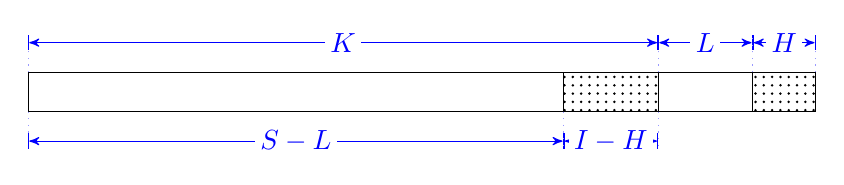
\begin{tikzpicture}
    \draw (0,0) rectangle +(10,0.5);
    \draw [pattern=dots] (8,0) rectangle +(-1.2,0.5);
    \draw [pattern=dots] (10,0) rectangle +(-0.8,0.5);
    
    \lineann[0.5]{(0,0.5)}{0}{8}{$K$};
    \lineann[0.5]{(8,0.5)}{0}{1.2}{$\ldpcnum{}$};
    \lineann[0.5]{(10,0.5)}{0}{-0.8}{$\hdpcnum{}$};
    \lineann[-0.5]{(0,0)}{0}{6.8}{$\smnum-\ldpcnum$};
    \lineann[-0.5]{(6.8,0)}{0}{1.2}{$\innum-\hdpcnum$};
  \end{tikzpicture}
  \caption{Packets partition}
  \label{fig:part}
\end{figure}

\subsection{Generator Matrices of Batches}
\label{sec:gener-matr-batch}

The generator matrix of a batch with degree $d$ is a $d\times M$
matrix. 

Though random generator matrices work well, we can still try to use deterministic generator matrices, which
has the advantage in term of less randomness. For degree $d < q$, we
can try to use a submatrix of Vandermonde matrix as a generator
matrix.

Let
\begin{equation*}
  V =
  \begin{bmatrix}
    1 & \alpha_1 & \alpha_1^2 & \cdots & \alpha_1^{M-1} \\
    1 & \alpha_2 & \alpha_2^2 & \cdots & \alpha_2^{M-1} \\
    \vdots & \vdots & \vdots & \ddots & \vdots \\
    1 & \alpha_d & \alpha_1^2 & \cdots & \alpha_d^{M-1} \\
  \end{bmatrix}
\end{equation*}
where $\alpha_i$, $i=1,\dots d$, are different non-zero field
elements of $GF(q)$.


\section{Inactivation Decoding}
\label{sec:inact}

\subsection{Received Packets Processing}

The received packets of a batch $i$ are given by
\begin{eqnarray*}
  \mathbf{Y}[i] 
  & = & \mathbf{B} [i] \mathbf{G}[i] \mathbf{H}[i] \\
  & = & \mathbf{B}_D [i] \mathbf{G}_D[i]\mathbf{H}[i] + \mathbf{B}_A [i] \mathbf{G}_A[i]\mathbf{H}[i] + \mathbf{B}_I [i] \mathbf{G}_I[i] \mathbf{H}[i]
\end{eqnarray*}
where $\mathbf{B}_D$, $\mathbf{B}_A$ and $\mathbf{B}_I$ are decoded,
active but undecoded and inactive packets. When a new packet
$\mathbf{Y}[i;k]$ with coding vector $\mathbf{H}[i;k]$ is received,
\begin{enumerate}
\item compute the active coefficients $\mathbf{C}_A[i;k]\leftarrow \mathbf{G}_A[i]\mathbf{H}[i;k]$,
\item compute the inactive coefficients $\mathbf{C}_I[i;k]\leftarrow \mathbf{G}_I[i]\mathbf{H}[i;k]$, and
\item compute the decoded coefficients $\mathbf{G}_D[i]\mathbf{H}[i;k]$ and substitute the decoded packets $\mathbf{B}_D [i] = \mathbf{Y}_{\mathbf{B}_D [i]} + \mathbf{B}_I \mathbf{C}_{\mathbf{B}_D [i]}$ as $\mathbf{Y}[i;k] \leftarrow \mathbf{Y}[i;k] - \mathbf{Y}_{\mathbf{B}_D [i]}\mathbf{G}_D[i]\mathbf{H}[i;k]$ and $\mathbf{C}_I[i;k] \leftarrow \mathbf{C}_I[i;k] + \mathbf{C}_{\mathbf{B}_D [i]}\mathbf{G}_D[i]\mathbf{H}[i;k]$.
\end{enumerate}


After the above computation and substitution, the effective received
packets are
\begin{equation*}
  \mathbf{Y}[i] = \mathbf{B}_A [i] \mathbf{C}_A[i] + \mathbf{B}_I \mathbf{C}_I[i]
\end{equation*}
where $\mathbf{B}_I$ is all the inactive packets.
Note that $\mathbf{B}_A[i]$ can be empty.


\subsection{Decoding a Batch}

If $\mathbf{C}_A[i]$ has full row rank, we can decode the batch by
applying Gaussian elimination such that $\mathbf{C}_A[i]
\rightarrow \begin{bmatrix} \mathbf{I} & \mathbf{0} \end{bmatrix}$ and
$\mathbf{Y}[i] = \mathbf{B}_A [i] \begin{bmatrix} \mathbf{I} & \mathbf{0} \end{bmatrix} + \mathbf{B}_I \mathbf{C}_I[i]$. Let
\begin{eqnarray*}
  \mathbf{Y}_1[i] & = & \mathbf{B}_A [i] + \mathbf{B}_I \mathbf{C}_1[i] \\
  \mathbf{Y}_2[i] & = & \mathbf{B}_I \mathbf{C}_2[i].
\end{eqnarray*}
After decoding all the batches, we obtain
\begin{equation*}
  \begin{bmatrix}
    \mathbf{B}_A & \mathbf{B}_I 
  \end{bmatrix}
  \begin{bmatrix}
    \mathbf{I} & \mathbf{0} & \mathbf{Q}_A\\
    \mathbf{C}_1 & \mathbf{C}_2 & \mathbf{Q}_I
  \end{bmatrix}
  = 
  \begin{bmatrix}
    \mathbf{Y}_1 & \mathbf{Y}_2 & \mathbf{0}
  \end{bmatrix}
\end{equation*}
where the $\mathbf{Q}_A$ and $\mathbf{Q}_I$ are submatrices of
$\mathbf{Q}$, which corresponds to the HDPC constraints.

\subsection{Decoding of Inactive Packets}
\label{sec:pre:inac:inac}

We can solve $\mathbf{B}_I$ by the following equation
\begin{equation*}
  \mathbf{B}_I 
  \underbrace{\begin{bmatrix}
    \mathbf{C}_2 & \mathbf{C}_1 \mathbf{Q}_A - \mathbf{Q}_I
  \end{bmatrix}}_{\mathbf{C}}
  = 
  \underbrace{\begin{bmatrix}
    \mathbf{Y}_2 & \mathbf{Y}_1\mathbf{Q}_A
  \end{bmatrix}}_{\mathbf{Y}}.
\end{equation*}
Only linearly independant columns of $\mathbf{C}_2$ are useful.

We can compute $\mathbf{C}_1 \mathbf{Q}_A+\mathbf{Q}_I$ and
$\mathbf{Y}_1\mathbf{Q}_A$ using
\begin{eqnarray*}
  \mathbf{C}_1 \mathbf{Q}_A + \mathbf{Q}_I & = &  
  \begin{bmatrix}
    \mathbf{C}_1 & \mathbf{I}
  \end{bmatrix}
  \begin{bmatrix}
    \mathbf{Q}_A \\ \mathbf{Q}_I
  \end{bmatrix}  \\
  \mathbf{Y}_1\mathbf{Q}_A & = & \tilde{\mathbf{Y}}_1\mathbf{Q},
\end{eqnarray*}
where if the $i$th variable node is invative, the $i$th column of
$\tilde{\mathbf{C}}_1$ is all zero, the $i$th column of $\mathbf{1}_I$
contains one $1$ in the position of the inactSeq of the $i$th variable
node, and the $i$th column of $\tilde{\mathbf{Y}}_1$ is all zero; if
the $i$th variable node is decoded, the $i$th column of
$\tilde{\mathbf{C}}_1$ is the corresponding column in $\mathbf{C}_1$,
the $i$th column of $\mathbf{1}_I$ is all zero, and the $i$th column
of $\tilde{\mathbf{Y}}_1$ is the corresponding column in
$\mathbf{Y}_1$.

An arbitrary matrix multiplying with $\mathbf{Q}$ can be computed easily.

\section{Other}

\subsection{Inductive Checking of Linear Independance}

Let $x_i$, $i=1,2,\cdots,$ be a sequence of vecotrs and $B_i$,
$i=0,1,\cdots,$ be a set of vectors defined as
\begin{eqnarray*}
  B_0 & = & \emptyset \\
  B_i & = & B_{i-1}\ \text{if}\ x_i\not\perp B_{i-1} \\
  B_i & = & B_{i-1}\cup\{x_i\}\ \text{if}\ x_i\perp B_{i-1}
\end{eqnarray*}
How to fast check whether $ x_i\perp B_{i-1}$ or not?

This algorithm is used in NCCoder and Decoder when receiving packets,
as wll as in inactive decoding.

\chapter{Implementations}

\section{BatsBasic Class}

\subsection{Member Variables}


\subsubsection{smNum}

\subsubsection{packets} \label{sec:bas:pkg}

\begin{lstlisting}
SymbolType * packets;  
\end{lstlisting}

Not allocated.

\subsubsection{checkPackets}\label{sec:bas:chpkg}

\begin{lstlisting}
SymbolType * checkPackets;  
\end{lstlisting}

Not allocated. 



\section{BatsEncoder Class}
\label{chap:enc}




\subsection{Member Functions}

\subsubsection{setInputPackets}

Flow chart in Fig.~\ref{flow:enc:set}.

\begin{figure}
  \centering

  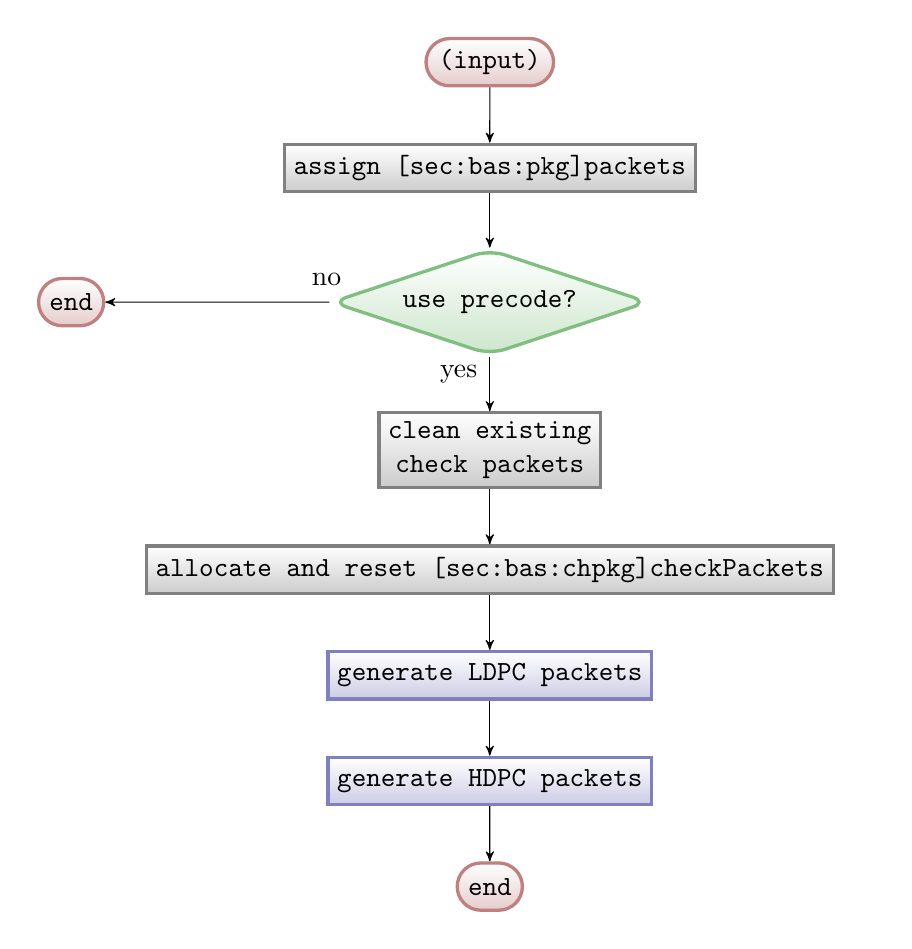
\begin{tikzpicture}
    \matrix[column sep=5mm, row sep=7mm] {
      % row 1
      & \node (s) [endblk] {(input)}; & \\
      % row 2
      & \node (nrec) [process] {assign \hyperref[sec:bas:pkg]{packets}}; &\\
      % row 3
      \node (enda) [endblk] {end};& 
      \node (check) [conditional] {use precode?}; & \\
      % row 4
      & \node (clean) [process] {clean existing\\ check packets}; &\\
      % row 5
      & \node (alloc) [process] {allocate and reset \hyperref[sec:bas:chpkg]{checkPackets}}; & \\
      % row 6
      & \node (ldpc) [subroutine] {generate LDPC packets}; & \\
      % row 7
      & \node (hdpc) [subroutine] {generate HDPC packets}; & \\
      % row 8
      & \node (endd) [endblk] {end};& \\
    };
    { [start chain]
      \chainin (s);
      \chainin (nrec) [join=by arrow];
      \chainin (check) [join=by arrow, lno, byes];
      { [start branch=end]
        \chainin (enda) [join=by arrow];
      }
      \chainin (clean) [join=by arrow];
      \chainin (alloc) [join=by arrow];
      \chainin (ldpc) [join=by arrow];
      \chainin (hdpc) [join=by arrow];
      \chainin (endd) [join=by arrow];
    }
  \end{tikzpicture}
  \caption{BatsEncoder::setInputPackets}
  \label{flow:enc:set}
\end{figure}

\subsubsection{genLdpc}


\subsubsection{genHdpc}


\subsubsection{genBatchWithKey}
\label{sec:enc:genbatch}

Flow chart in Fig.~\ref{flow:enc:batch}.

\begin{figure}
  \centering

  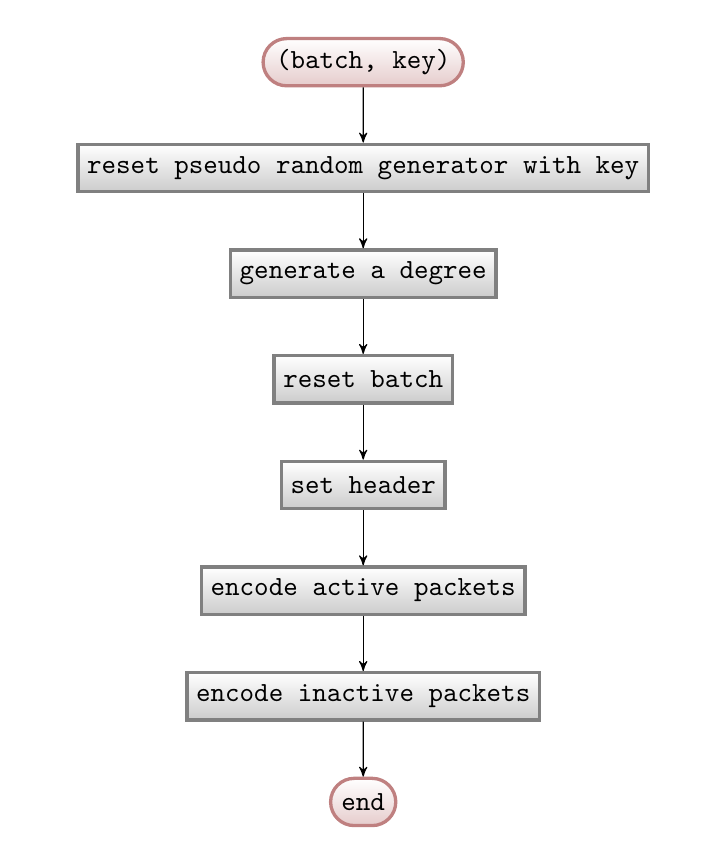
\begin{tikzpicture}
    \matrix[column sep=5mm, row sep=7mm] {
      % row 1
      & \node (s) [endblk] {(batch, key)}; & \\
      % row 2
      & \node (seed) [process] {reset pseudo random generator with key}; &\\
      % row 3
      & \node (degree) [process] {generate a degree}; & \\
      % row 4
      & \node (reset) [process] {reset batch}; & \\
      % row 5
      & \node (header) [process] {set header}; & \\
      % row 6
      & \node (bats) [process] {encode active packets}; & \\
      % row 7
      & \node (inact) [process] {encode inactive packets}; & \\
      % row 8
      & \node (endd) [endblk] {end}; &\\
    };
    { [start chain, every on chain/.style={join=by arrow}]
      \chainin (s);
      \chainin (seed);
      \chainin (degree);
      \chainin (reset);
      \chainin (header);
      \chainin (bats);
      \chainin (inact);
      \chainin (endd);
    }
  \end{tikzpicture}
  \caption{BatsEncoder::genBatchWithKey}
  \label{flow:enc:batch}
\end{figure}


\section{VariableNode Class}
\label{sec:varnode}

\subsection{Member Variables}

\subsubsection{$inactSeq$}

The initial value of $inactSeq$ is $-1$. For IN packets, their
$inactSeq$ are assigned to be from $0$ to $piNum-1$.  When a new
variable node is inactivated, its $inactSeq$ is the current number of
inactive variable nodes (excluding itself).

In the matrix $\mathbf{B}_I$, the $i$th column corresponds to the
variable node with $inactSeq = i$. So $inactSeq$ is used to access the
corresponding inactivation coefficients. 

\section{CheckNode Class}
\label{sec:check}




\section{BatsDecoder Class}
\label{sec:decoder}

\subsection{Using a Decoder}

Fig.~\ref{flow:dec:use} illustrates a type flow to perform
inactivation decoding.

\begin{figure}
\centering
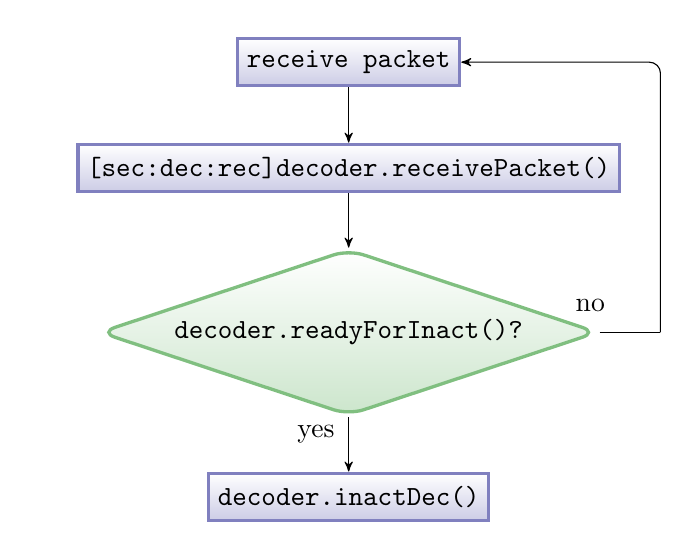
\begin{tikzpicture}
  \matrix[column sep=5mm, row sep=7mm] {
    % row 1
    & \node (rec) [subroutine] {receive packet}; & \\
    % row 2
    & \node (call) [subroutine] {\hyperref[sec:dec:rec]{decoder.receivePacket()}}; & \\
    % row 3
    & \node (ready) [conditional] {decoder.readyForInact()?}; 
    & \node (point) [point] {}; \\
    % row 4
    & \node (inact) [subroutine] {decoder.inactDec()}; & \\
  };

  { [start chain]
    \chainin (rec);
    \chainin (call) [join=by arrow];
    \chainin (ready) [join=by arrow, rno, byes];
    { [start branch=no]
      \chainin (point) [join];
      \chainin (rec) [join=by {vh path, arrow}];
    }
    \chainin (inact) [join=by arrow];
      
   }
   
\end{tikzpicture}
\caption{A typical flow to use an instance decoder of BatsDecoder.}
\label{flow:dec:use}
\end{figure}


\subsection{Member Variables}


\subsubsection{nRecPkg} \label{sec:dec:nrecpkg} 

Number of the packets received. Used to decide when to start
inactivation decoding.

\subsubsection{nRecBatch} \label{sec:dec:nrecbatch} 

An upper bound on the number of the batches received. 
Used to get the rank distribution of received batches.


\subsubsection{nC2, maxC2, C and Y}

Ref Section~\ref{sec:pre:inac:inac}. C and Y are matrices of
maxInact+maxRedun columns. The first maxC2 (= maxInact+maxRedun - hdpcNum) columns of C and Y are used
for $\mathbf{C}_2$ and $\mathbf{Y}_2$, respectively. nC2 $\leq$ maxC2
is the actual number of columns in $C_2$. The $i$ column of
$\mathbf{C}_2$ is saved in C[maxC2-1-i].


\subsubsection{Decoder Status}

The following are some constant of decoder.
\begin{description}
\item[$totalNum$] the total number of packets including input and check packets.
\end{description}
The following are variables of decoder status.
\begin{description}
\item[$nRecPkg$] the number of packets received (after checking linear independance).
\item[$nDecoded$] the number of decoded packets (including check packets).
\item[$nC2$] the number of packets in $C_2$ (after checking linear independance).
\item[$nInactVar$] the number of inactive nodes.
\end{description}


\subsection{Member Functions}

\subsubsection{receivePacket}
\label{sec:dec:rec}

Flow chart is in Fig.~\ref{flow:dec:rec}.

\begin{figure}
\centering
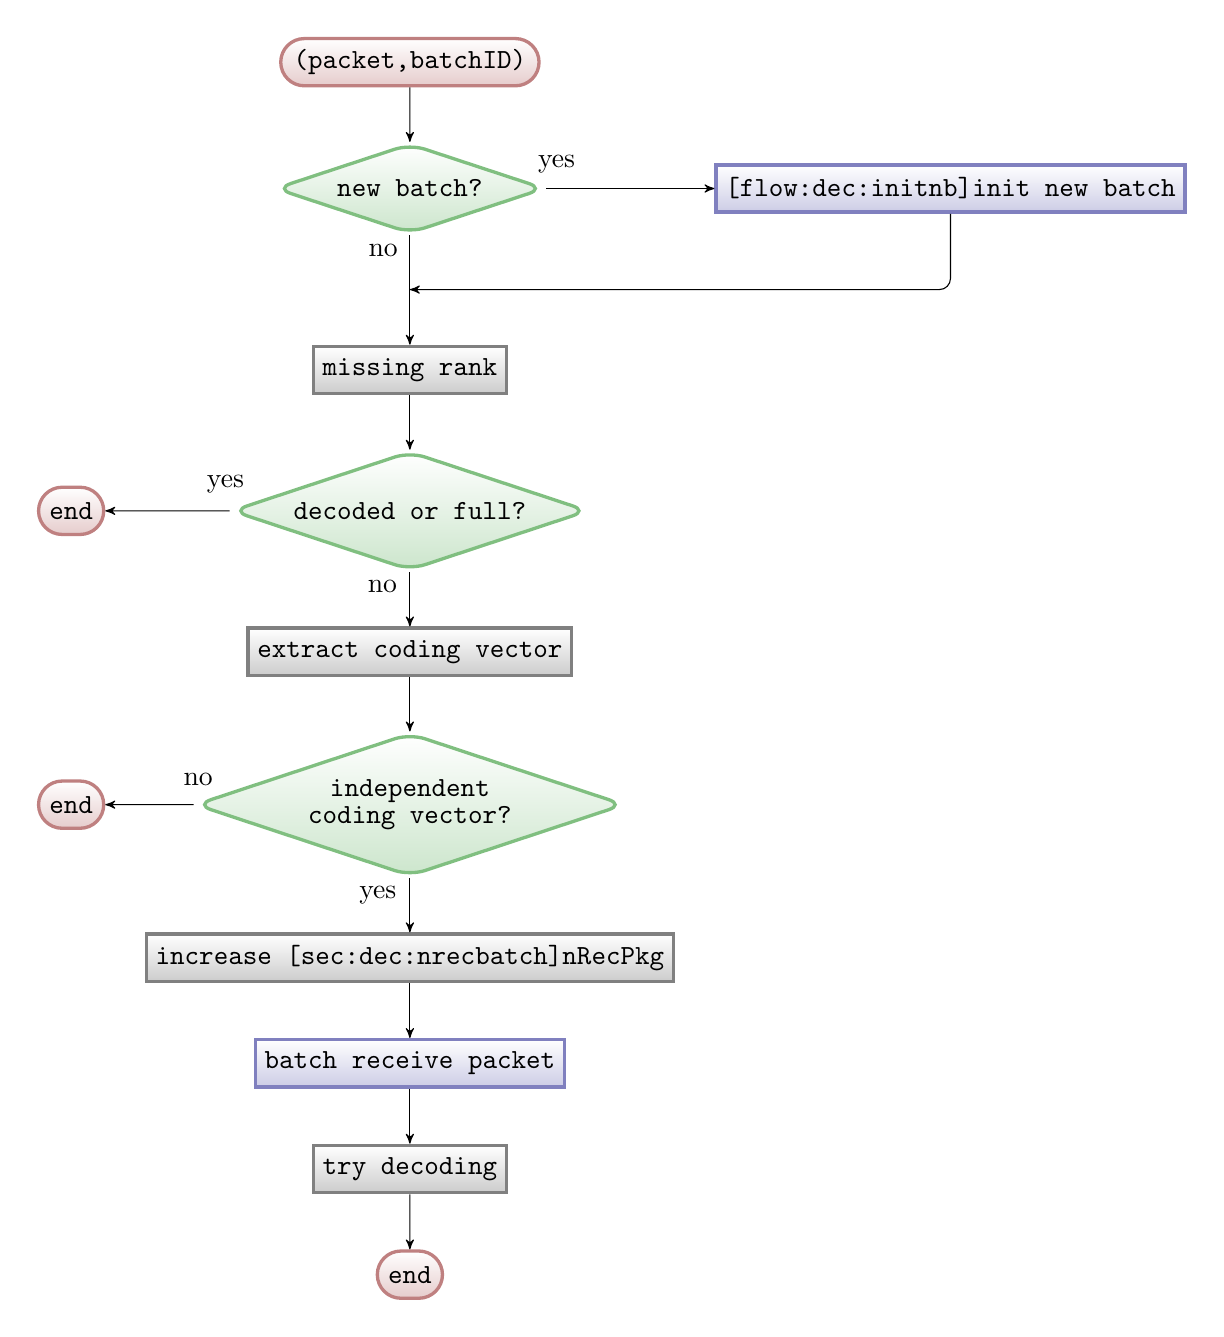
\begin{tikzpicture}
  \matrix[column sep=5mm, row sep=7mm] {
    % row 1
    & \node (s) [endblk] {(packet,batchID)}; & \\
    % row 3
    & \node (nb) [conditional] {new batch?}; & 
    \node (ynb) [subroutine] {\hyperref[flow:dec:initnb]{init new batch}}; \\
    % row 3a
    & \node (p1) [point] {}; & \\
    % row 4
    & \node (miss) [process] {missing rank}; & \\
    % row 5
    \node (enda) [endblk] {end}; & 
    \node (dec) [conditional] {decoded or full?}; & \\
    % row 5a
    & \node (ext) [process] {extract coding vector}; & \\
    % row 5b
    \node (endb) [endblk] {end}; & 
    \node (ind) [conditional] {independent\\[-2pt] coding vector?}; & \\
    % row 6
    & \node (aa) [process] {increase \hyperref[sec:dec:nrecbatch]{nRecPkg}}; & \\
    % row 6a
    & \node (rec) [subroutine] {batch receive packet}; & \\
    % row 7
    & \node (try) [process] {try decoding}; & \\
    % row 8
    & \node (endd) [endblk] {end}; &\\
  };

  { [start chain]
    \chainin (s);
    \chainin (nb) [join=by arrow, ryes, bno];
    { [start branch=init new]
      \chainin (ynb) [join=by arrow];
      \chainin (p1) [join=by {vh path, arrow}];
    }
    \chainin (p1) [join];
    \chainin (miss) [join=by arrow];
    \chainin (dec) [join=by arrow, lyes, bno];
    { [start branch=end]
      \chainin (enda) [join=by arrow];
    }
    \chainin (ext) [join=by arrow];
    \chainin (ind) [join=by arrow, lno, byes];
    { [start branch=end]
      \chainin (endb) [join=by arrow];
    }
    \chainin (aa) [join=by arrow];
    \chainin (rec) [join=by arrow];
    \chainin (try) [join=by arrow];
    \chainin (endd) [join=by arrow];
   }
   
\end{tikzpicture}
\caption{BatsDecoder::receivePacket}
\label{flow:dec:rec}
\end{figure}

\subsubsection{initNewBatch}
\label{sec:dec:initnb}

This function is similar to \hyperref[sec:enc:genbatch]{BatsEncoder::genBatchWithKey}.

\begin{figure}
  \centering
  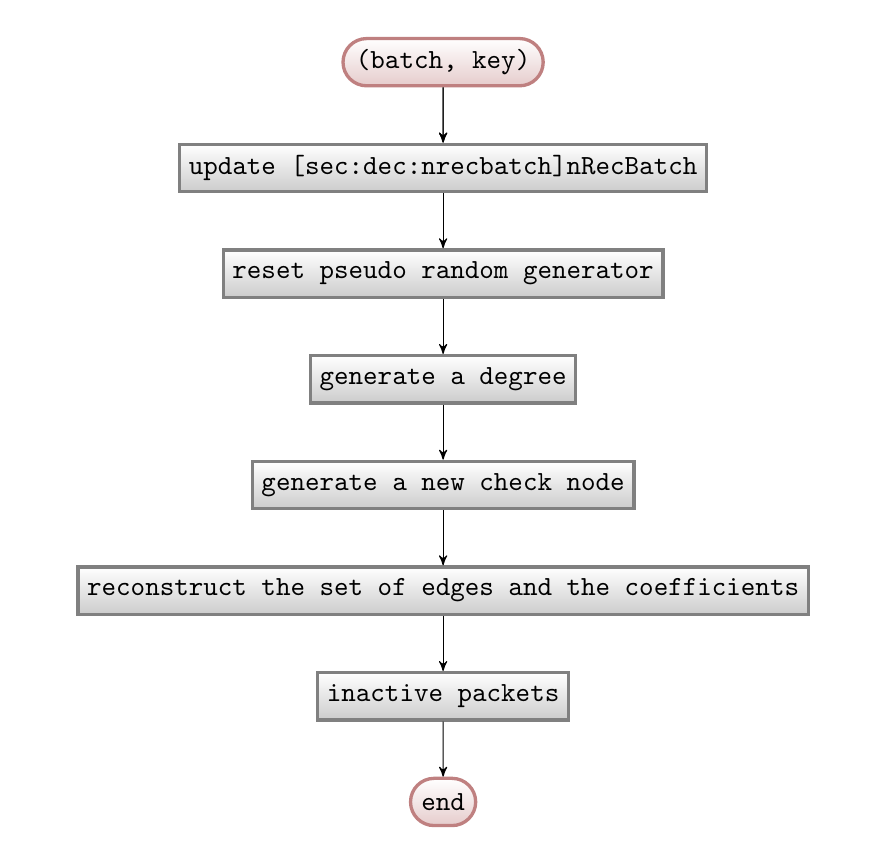
\begin{tikzpicture}
    \matrix[column sep=5mm, row sep=7mm] {
      % row 1
      & \node (s) [endblk] {(batch, key)}; & \\
      % row 1a
      & \node (nrec) [process] {update \hyperref[sec:dec:nrecbatch]{nRecBatch}}; &\\
      % row 2
      & \node (seed) [process] {reset pseudo random generator}; &\\
      % row 3
      & \node (degree) [process] {generate a degree}; & \\
      % row 3a
      & \node (check) [process] {generate a new check node}; & \\
      % row 6
      & \node (bats) [process] {reconstruct the set of edges and the coefficients}; & \\
      % row 7
      & \node (inact) [process] {inactive packets}; & \\
      % row 8
      & \node (endd) [endblk] {end}; &\\
    };
    { [start chain, every on chain/.style={join=by arrow}]
      \chainin (s);
      \chainin (nrec) [join=by arrow];
      \chainin (seed);
      \chainin (degree);
      \chainin (check);
      \chainin (bats);
      \chainin (inact);
      \chainin (endd);
    }
  \end{tikzpicture}
  \caption{BatsDecoder::initNewBatch}
  \label{flow:dec:initnb}
\end{figure}


\chapter{Testing}
\label{chap:test}

\section{No HDPC and PI}

In class BatsBasic, set $hdpcNum = 0$ and $piNum = hdpcNum$.

\section{To Fix}

\subsection{Reduce Packet Drop}

Received packets of decoded batches can still be put in $C_2$.

\subsection{LDPC}

Now there are many undecoded LDPC symbols after all batches are
decoded. We can try use smaller degree of LDPC symbols, or using the
idea of batched LDPC.

\subsection{Redesign CheckNode}


\begin{thebibliography}{99}
\bibitem{rfc6330} 
  http://tools.ietf.org/pdf/rfc6330.pdf
\end{thebibliography}


\end{document}


